\chapter[Resultados e Discussões]{Resultados}

\section{Solução Desenvolvida}

\subsection{Tecnologias e ferramentas utilizadas}
\label{sec:tecnologias_ferramentas}

Para a construção da proposta de solução final foram utilizadas algumas ferramentas, tecnologias e bibliotecas ao longo do processo de desenvolvimento. A seguir estas estão elencadas junto com a motivação de sua utilização dentro da solução:

    \begin{quote}
    \begin{itemize}
        \item ReactJS: Biblioteca javascript utilizada para criar a interface dos diferentes módulos da solução.
        \item Material UI: Biblioteca de componentes ReactJS para um desenvolvimento ágil e fácil, sendo utilizado para criar um visual mais agradável para a aplicação.
        \item Web3.Js: Coleção de bibliotecas que possibilitam a interação com nós ethereum remotos, utilizando conexões HTTP ou ICP. Possibilitando assim que os clientes possam se comunicar com o contrato inteligente desenvolvido.
        \item Metamask: Extensão de navegador para acesso a aplicativos distribuídos(Dapps), onde a mesma injeta a API Ethereum do Web3 no contexto javascript dos sites. Também permite que os usuários criem e gerenciem suas próprias identidades e transações, trazendo uma interface segura para revisar transações antes de aceitá-las ou rejeitá-las.
        \item Docker e Docker-compose: Containers utilizados para facilitar o gerenciamento de dependências da aplicação assim como orquestrar facilmente os ambientes de desenvolvimento e produção das mesmas.
        \item TESTNET Ropsten (ETH): Rede ethereum que executa o mesmo protocolo que o Ethereum(main net) e é usada para fins de teste. O contrato inteligente da solução está registrado nesta e rede e todas as transações ocorrem em interações dentro dela.
        \item Ropsten Ethereum Faucet: Ferramenta utilizada para obter ethers gratuitos da rede de testes Ropstas para as contas utilizadas na solução;
        \item Digital Ocean: Serviço de hospedagem utilizado para hospedar os módulos(Dapps) desenvolvidos em um servidor, possibilitando que as aplicações possam ser acessadas sem a necessidade de executá-las localmente.
        \item Solidity: Linguagem de programação de alto nível por meio da qual é possível criar aplicações descentralizadas, em especial os smart contracts, na Ethereum. 
        \item Truffle: Um ambiente de desenvolvimento, framework de testes e pipeline de ativos para blockchains usando a Ethereum Virtual Machine (EVM). Tendo sido utilizado principalmente na fase inicial de construção do contrato inteligente, possibilitando o desenvolvimento do mesmo mais rapidamente.
        \item Ganache: Blockchain Ethereum pessoal utilizado executar testes, executar comandos e inspecionar o estado enquanto controla como a cadeia de blocos opera localmente.
    \end{itemize}
    \end{quote}
        
        
\subsection{Arquitetura da Solução}

A solução foi desenvolvida seguindo uma arquitetura cliente-servidor, representada na Figura \ref{fig:dapp_arquitetura_solucao}. A parte do cliente nesta solução é composto pelas aplicações descentralizadas(Dapps) desenvolvidas, onde um módulo corresponde ao sistema utilizado pelas autoridades de trânsito e o outro módulo sendo o sistema de acesso dos motoristas. Já o servidor da solução corresponde a rede ethereum onde o \verb|deploy| do contrato inteligente foi feito e as transações são validadas pelos nós mineradores da rede, representado na Figura \ref{fig:dapp_rede_ethereum}.

    \begin{figure}[h]
         \centering
         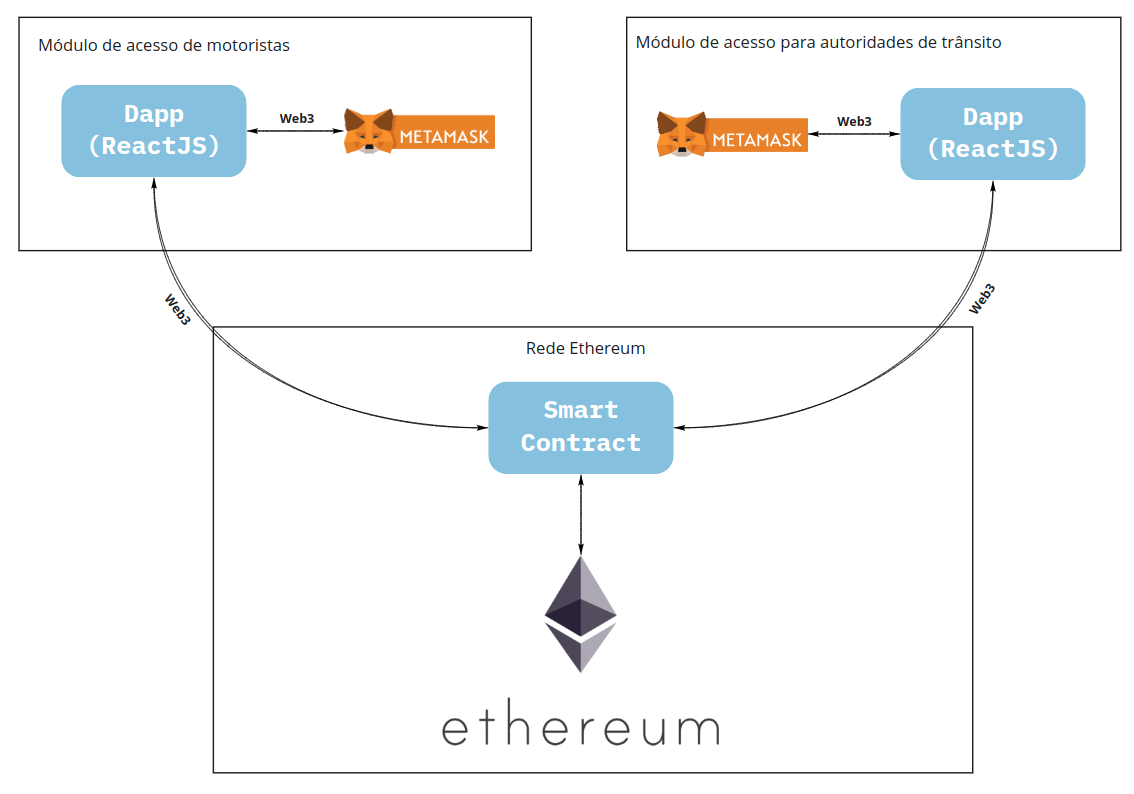
\includegraphics[scale=0.35]{figuras/capitulo_5/arquitetura_solucao.png}
         \caption{Representação da interação entre os módulos da solução - Imagem própria.}
         \label{fig:dapp_arquitetura_solucao}
    \end{figure}
                                                        
    \begin{figure}[h]
         \centering
         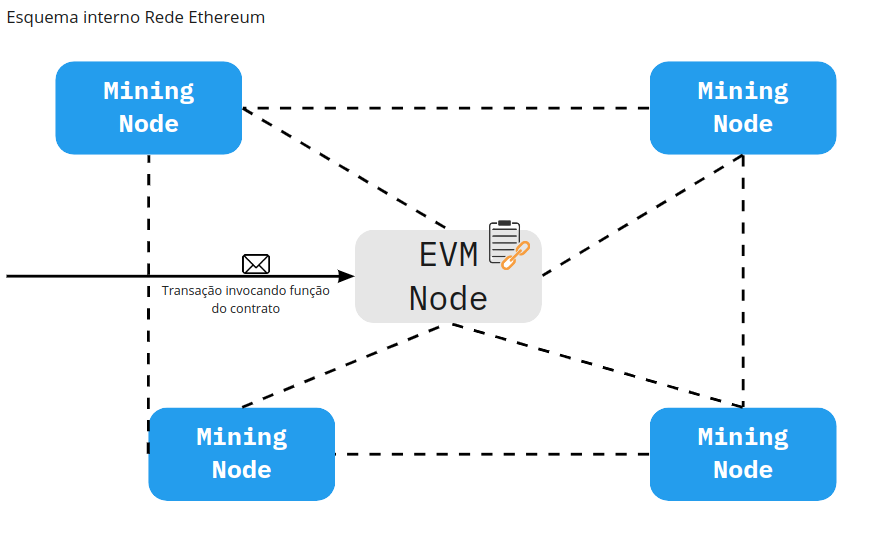
\includegraphics[scale=0.4]{figuras/capitulo_5/esquema_rede_ethereum.png}
         \caption{Representação da rede onde o contrato está na Ethereum Virtual Machine - Imagem própria.}
         \label{fig:dapp_rede_ethereum}
    \end{figure}
    
A rede ethereum atualmente utilizada para validar o protótipo e solução desenvolvida é a rede de testes Ethereum Ropsten. A rede de testes Ropsten é executada utilizando os mesmos protocolos da rede principal Ethereum, porém sem custos financeiros atrelados a seu funcionamento podendo assim que testes sejam realizados sem a aquisição de Ethers. A rede provê por meio dos Faucets  a possibilidade dos usuários obterem Ethers de forma gratuita e poderem assim usufruir de todas as funcionalidades da rede como realizar transações, deploy de smart contracts, envio de ethers e etc.

\subsection{Módulos do Sistema}

A solução do sistema é composta por dois diferentes módulos, um para acesso do usuário motorista e outro para acesso das autoridades de trânsito. Cada módulo desse sistema corresponde a uma aplicação, sendo estas executadas de forma paralela.

As funcionalidades do sistema possuem especificidades de acordo com o perfil de usuário que está utilizando o sistema, o que demanda um nível de autenticação para acesso a estas informações. A proposta de trabalho traz algumas premissas, onde as premissas II e IV indicam que  usuário do sistema seja ele um motorista ou autoridade de trânsito possui uma conta e uma única chave de acesso que o representa. Para realizar a autenticação dentro dos módulos do sistema, estas premissas são utilizadas como base e ocorre utilizando-se esta chave única.

\subsection{Autenticação dos usuários nos módulos sistema}

A autenticação nas aplicações não ocorre por meio de login e senha como usualmente em sistemas. Nesta solução a autenticação é feita com o auxílio da extensão metamask. Optou-se por esta abordagem para que o usuário tenha suas informações ainda mais resguardadas sem a necessidade de armazená-las em um local externo, garantindo assim que o princípio confidencialidade da segurança computacional definido por Stallings esteja presente em meio as aplicações.

O fluxo de autenticação ocorre da seguinte maneira em meio as aplicações:

    \begin{quote}
        \begin{enumerate}
            \item Quando o usuário requisita acesso a uma página do sistema, conta ativa no momento na extensão metamask é obtida com auxílio da extensão Web3;
            \item É feita uma chamada de função ao smart contract onde é verificado se esta conta existe em meio aos arrays de motorista ou autoridades de trânsito de acordo com o módulo acessado;
            \item Se a conta está presente no array solicitado a página é renderizada e o usuário está assim autorizado no sistema. No caso de negativa desta condição o usuário não é autorizado e não consegue acessar as funcionalidades do sistema.
        \end{enumerate}
    \end{quote}

\subsection{Autorização dentro do smart contract}

Na aplicação possuímos um esquema de autenticação de forma a garantir que somente pessoas autorizadas possuam acesso a determinadas funcionalidades, porém como garantir que isso também ocorra dentro do smart contract que é público dentro da rede

Dentro da rede Ethereum caso uma pessoa tenha o endereço do contrato o mesmo poderá visualizar todas as transações realizadas, assim como realizar chamadas de funções declaradas como públicas no código fonte caso tenha o conhecimento de sua declaração.

Como qualquer pessoa pode interagir com este contrato na rede pública existe outra camada de autenticação dentro das funções públicas desenvolvidas no contrato, onde caso a condição determinada não seja atendida a execução da função solicitada é interrompida. Este controle é feito utilizando a função \textit{require()} presente na linguagem solidity, onde é verificado se o endereço(\textit{address}) da conta \textit{sender} está registrado e autorizado a realizar o procedimento solicitado como no caso do registro de infrações de trânsito que só podem ser feitas por uma conta registrada com o perfil de autoridade de trânsito.


\subsection{Funcionalidades}

A proposta de solução elencou na Seção \ref{section:funcionalidades_propostas} algumas funcionalidades a serem desenvolvidas de forma a solucionar o problema levantado no desenvolvimento deste trabalho. A solução desenvolvida conseguiu contemplar todas estas funcionalidades propostas e consideradas fundamentais para o funcionamento do sistema RENAINF, demonstrando a possibilidade de adaptação de um sistema existente utilizando-se a tecnologia blockchain.

Porém tornou-se necessário uma adaptação na funcionalidade de Recurso / Cancelamento de infração de trânsito proposta inicialmente. Ao se mapear os requisitos de forma que essa atenda ao RENAINF e o CTB, ocorreu um erro de interpretação onde a proposta trazia inicialmente que a autoridade de trânsito que realizou o registro da infração seria também responsável por julgar este recurso e isto acaba não seguindo totalmente o processo adotado no código CTB. O Artigo 287 do CTB diz que uma junta de trânsito (Jari) será responsável pelo julgamento do recurso proposto e não a autoridade que registrou a infração, então foi necessário esta adaptação nos requisitos iniciais.

Para o funcionamento desta funcionalidade na solução atual a Jari é considerada uma autoridade de trânsito, que só possui acesso a essa funcionalidade, e é única em todo o sistema. Atualmente, todos os recursos realizados pelos motoristas são direcionados a essa única Jari registrada previamente na criação do contrato, atendendo assim o que está registrado no CTB e corrigindo o requisito errôneo mapeado anteriormente.

\subsubsection{Aplicação desenvolvida}

Para exemplificar do funcionamento dos módulos da aplicação cliente a seguir será descrito o processo para o registro de uma infração de trânsito realizado por uma autoridade de trânsito

    \begin{figure}[H]
         \centering
         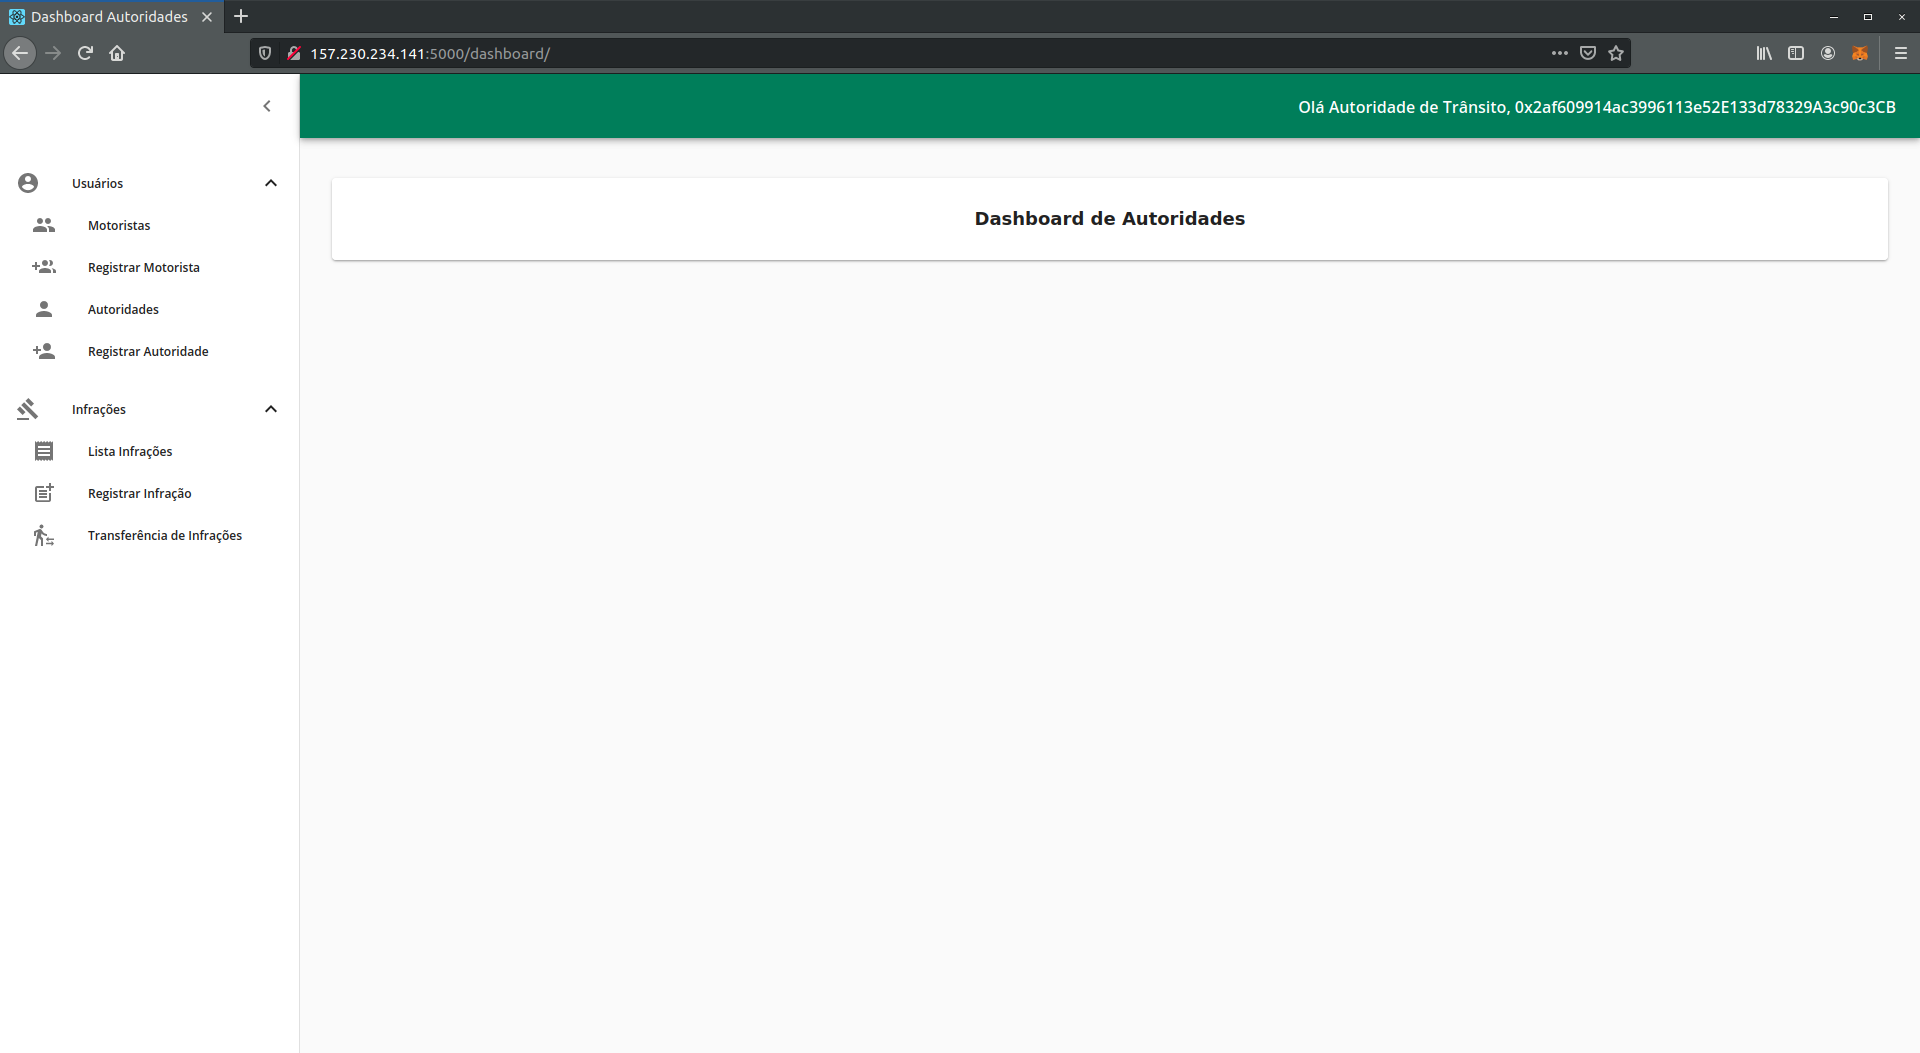
\includegraphics[scale=0.2]{figuras/capitulo_5/registro/print_1.png}
         \caption{Autoridade de Trânsito acessa o módulo exclusivo para autoridades de trânsito com a sua carteira autenticada}
         \label{fig:dapp_rede_ethereum}
    \end{figure}
 
    \begin{figure}[H]
         \centering
         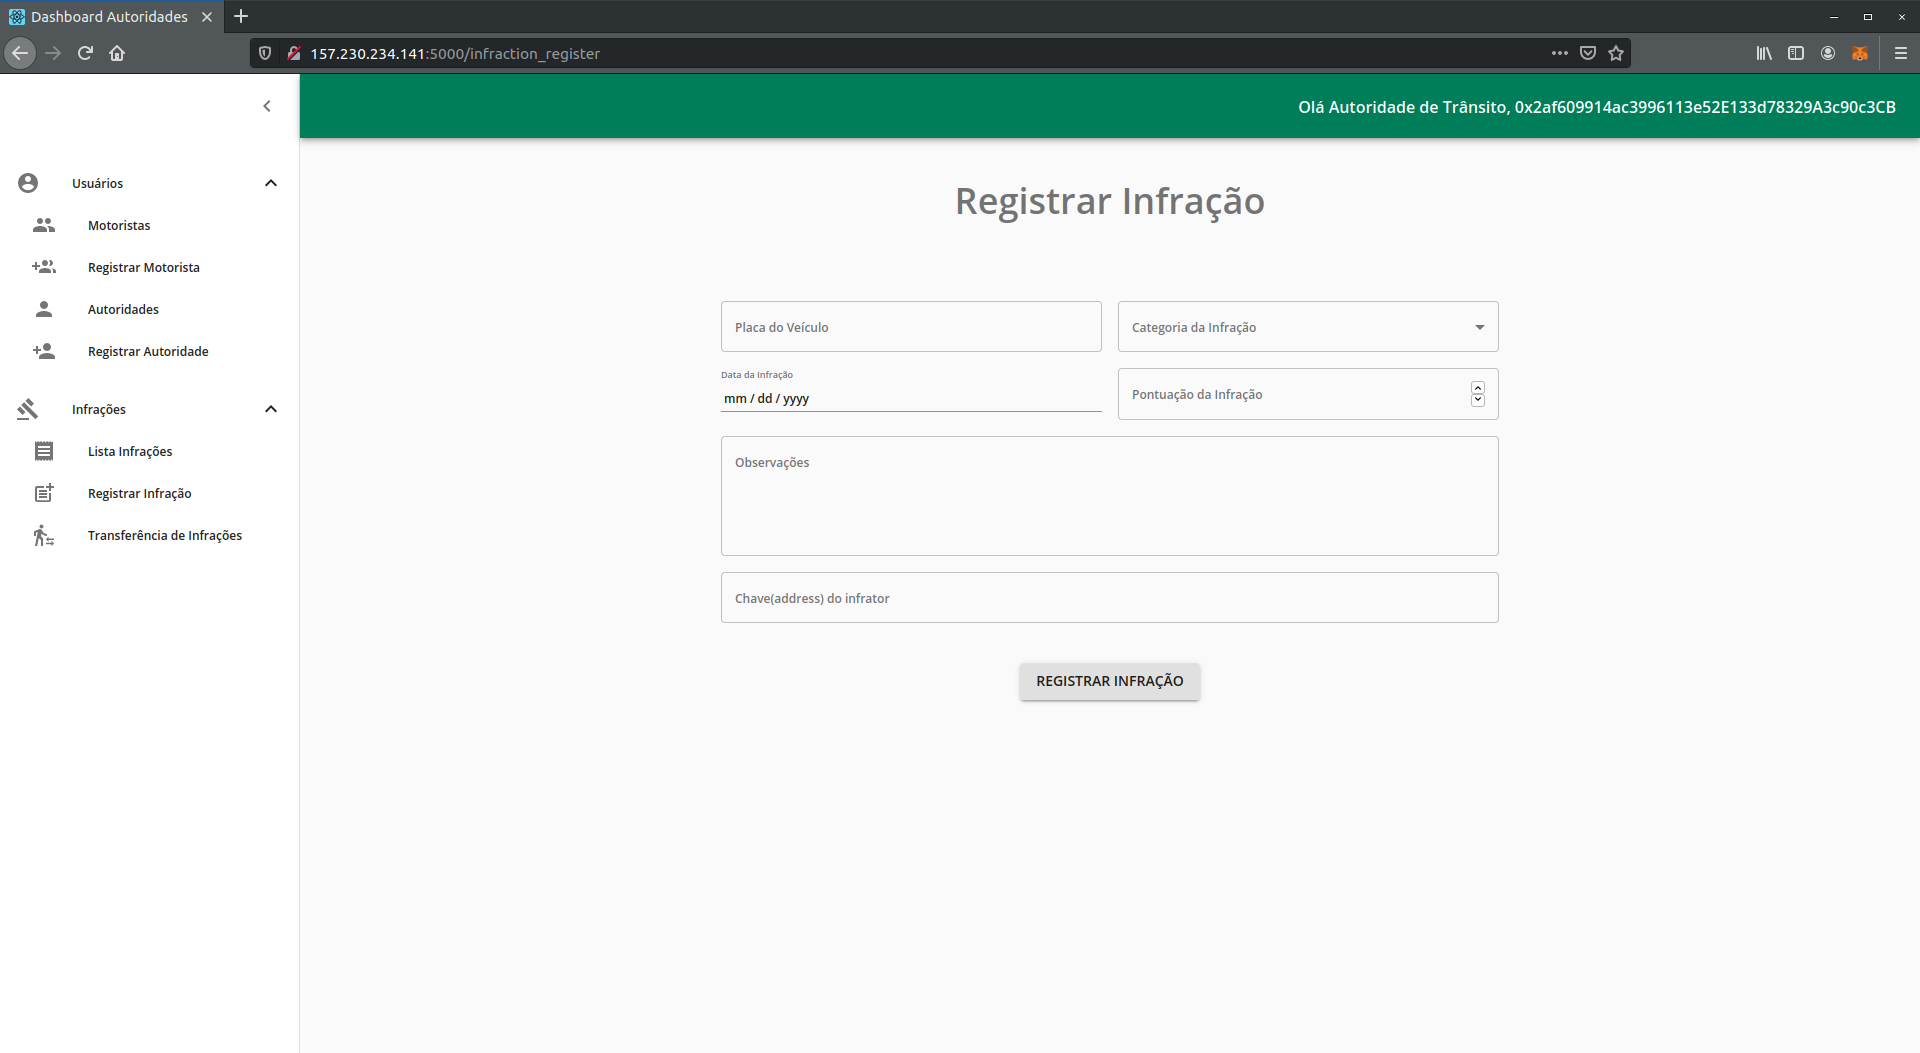
\includegraphics[scale=0.2]{figuras/capitulo_5/registro/print_2.png}
         \caption{A página contendo o formulário para registro é acessada utilizando o menu lateral}
         \label{fig:dapp_rede_ethereum}
    \end{figure}
    
    \begin{figure}[H]
         \centering
         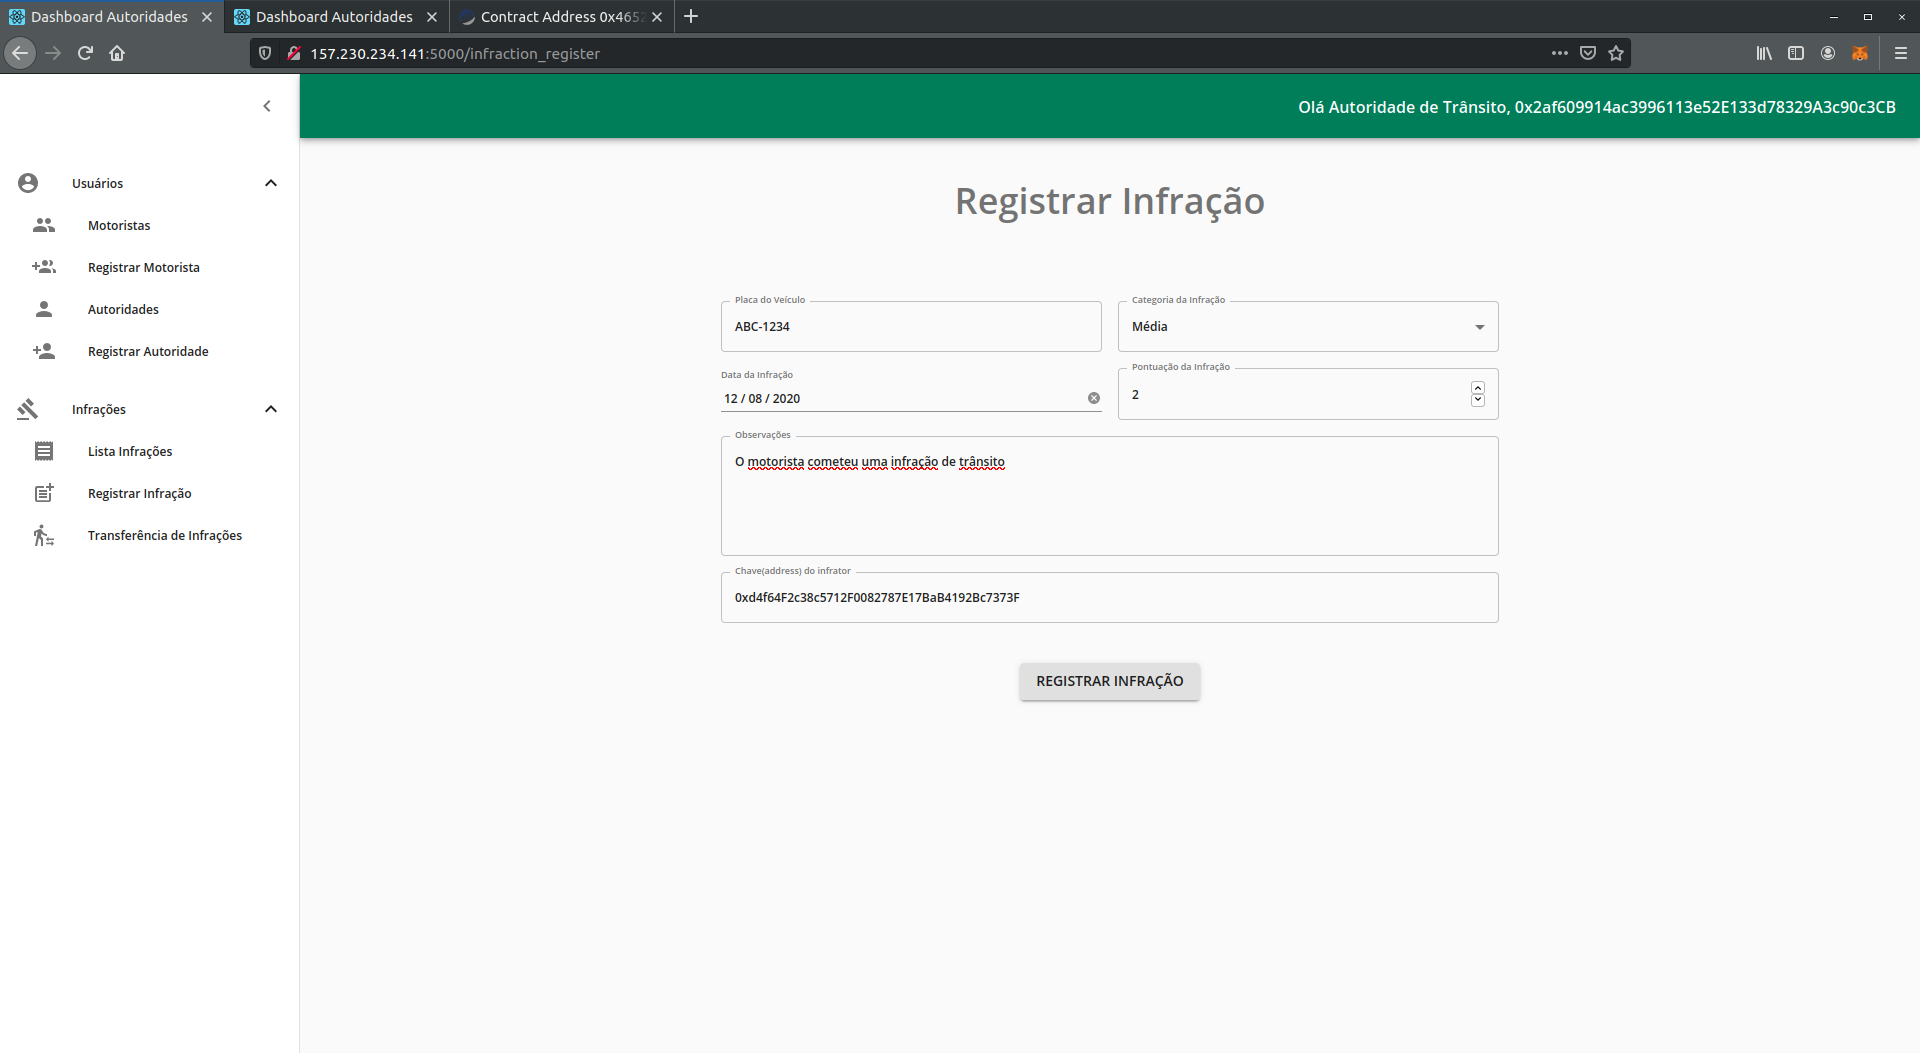
\includegraphics[scale=0.2]{figuras/capitulo_5/registro/print_3.png}
         \caption{As informações são preenchidas e o botão Registrar Infração é clicado.}
         \label{fig:dapp_rede_ethereum}
    \end{figure}
    
    \begin{figure}[H]
         \centering
         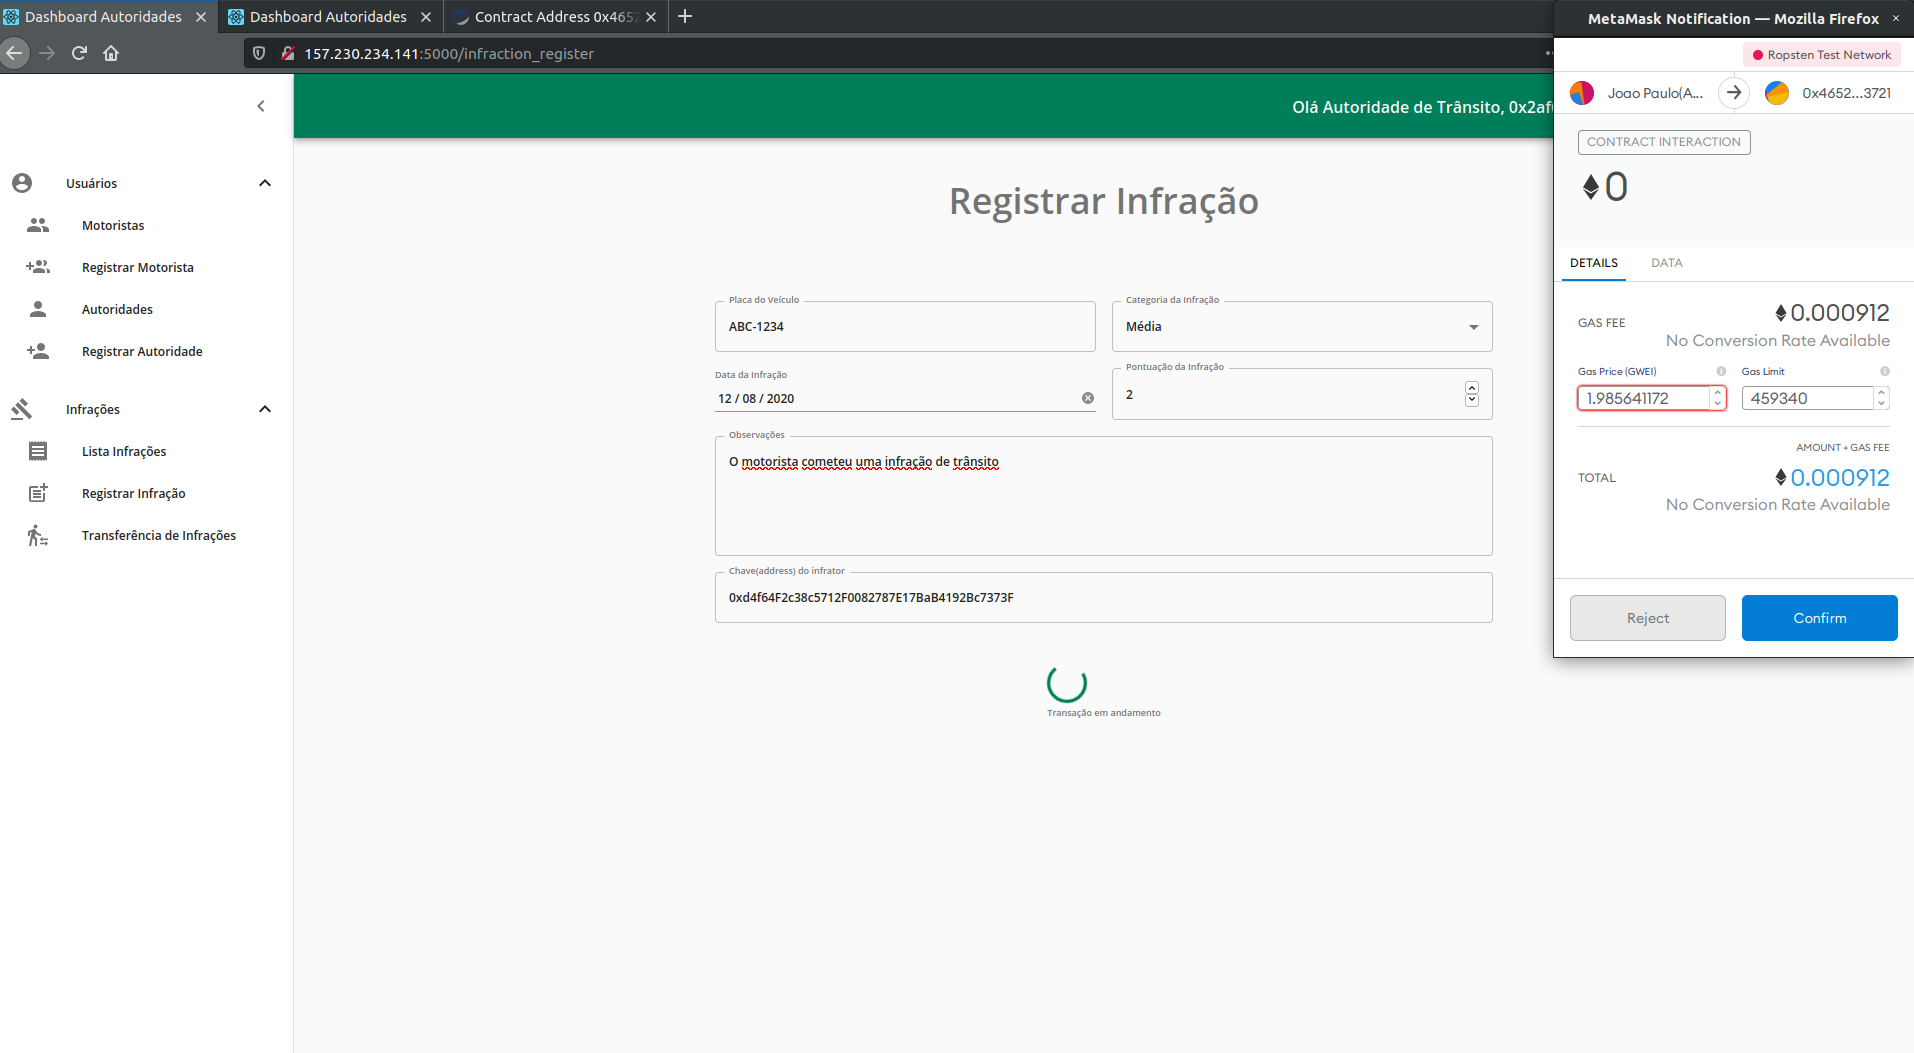
\includegraphics[scale=0.2]{figuras/capitulo_5/registro/print_4.png}
         \caption{A transação é assinada utilizando a carteira Metamask}
         \label{fig:dapp_rede_ethereum}
    \end{figure}
    
    \begin{figure}[H]
         \centering
         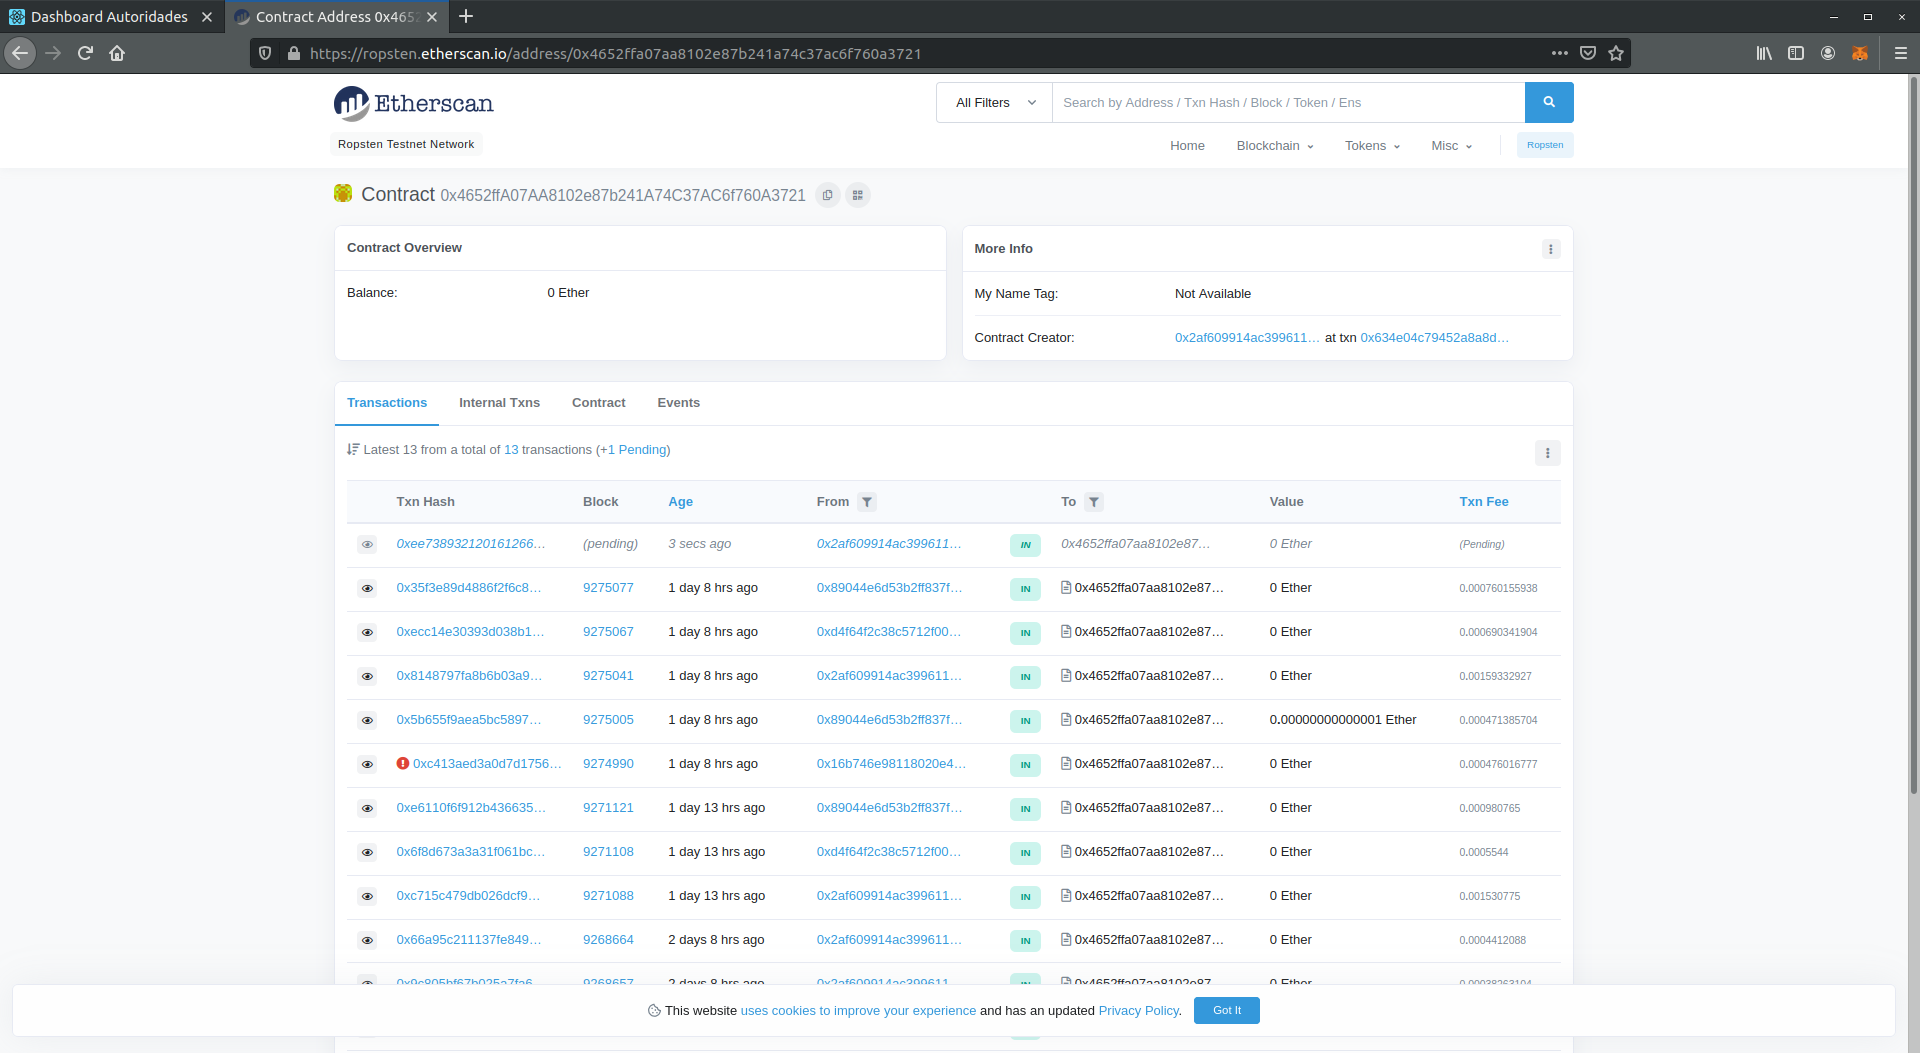
\includegraphics[scale=0.2]{figuras/capitulo_5/registro/print_5.png}
         \caption{Uma nova transação é criada para ser validada na rede blockchain.}
         \label{fig:dapp_rede_ethereum}
    \end{figure}
    
    \begin{figure}[H]
         \centering
         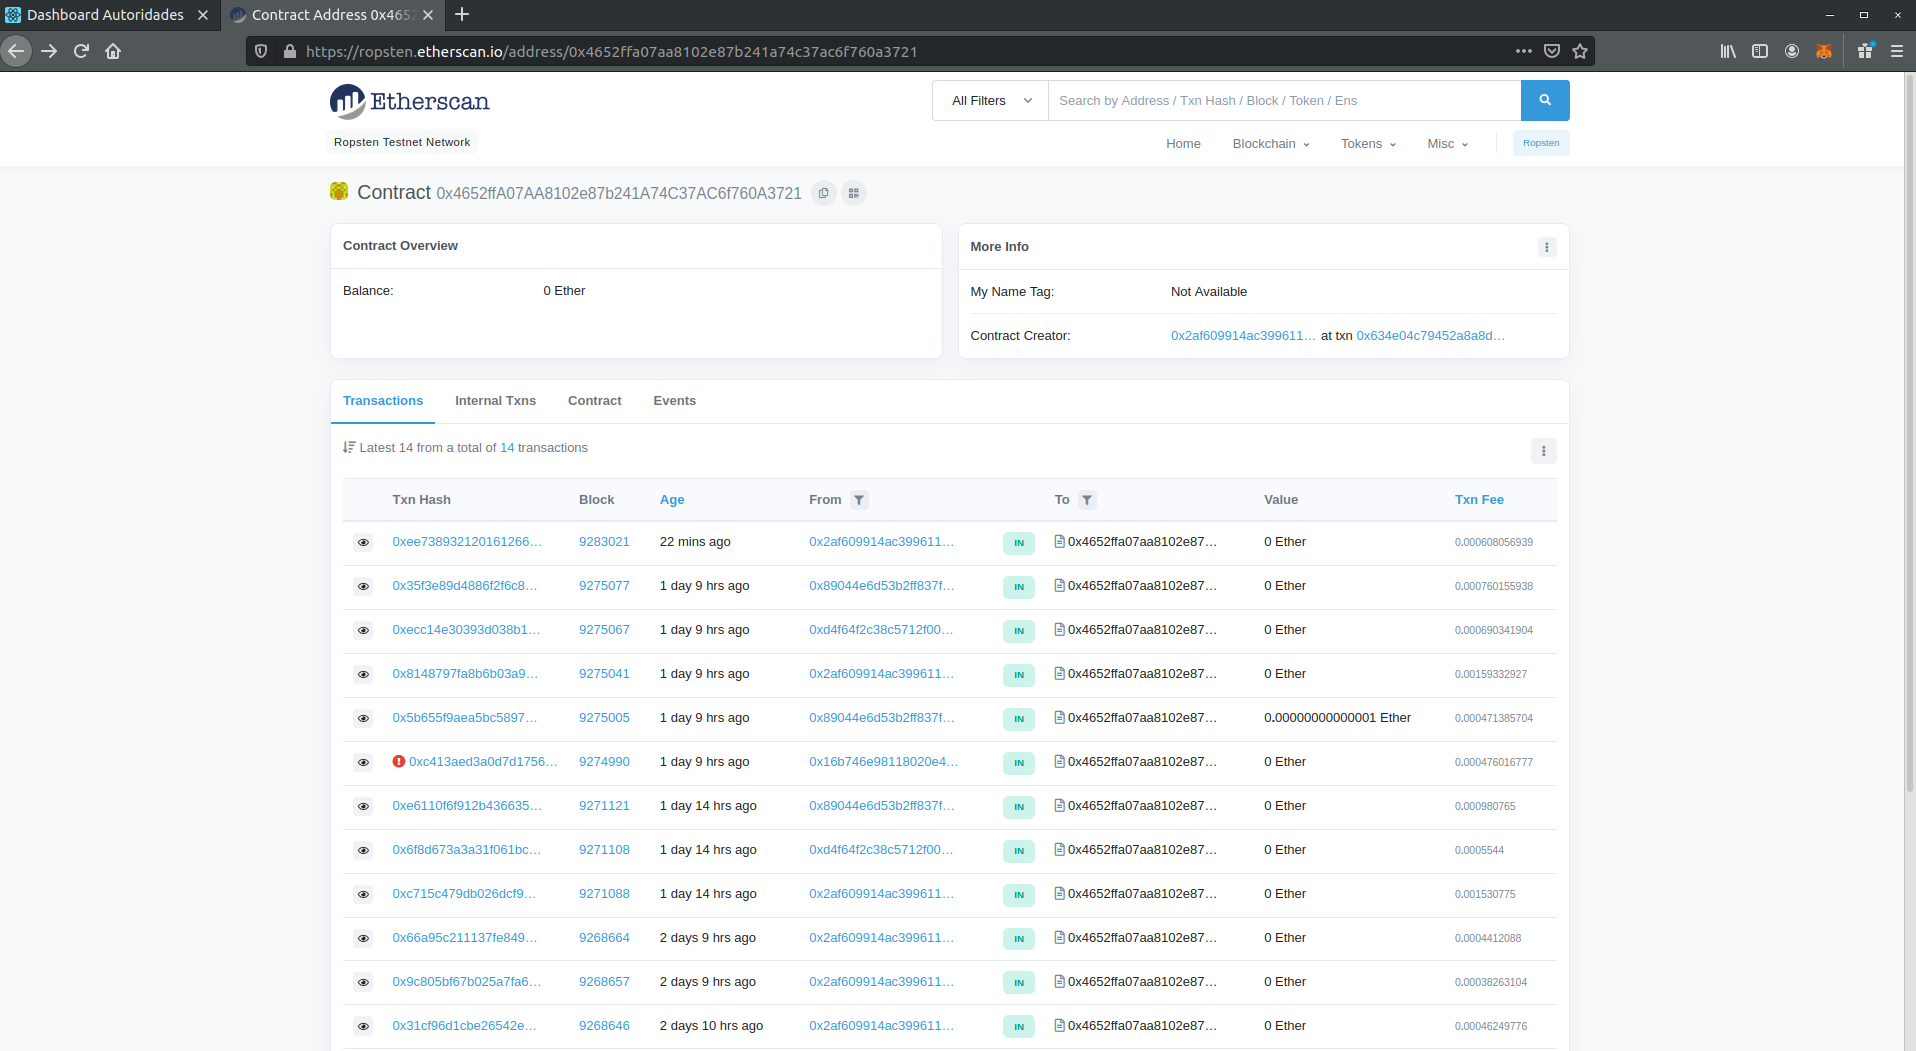
\includegraphics[scale=0.2]{figuras/capitulo_5/registro/print_6.png}
         \caption{Transação confirmada com sucesso e inserida na blockchain}
         \label{fig:dapp_rede_ethereum}
    \end{figure}
    
    
    \begin{figure}[H]
         \centering
         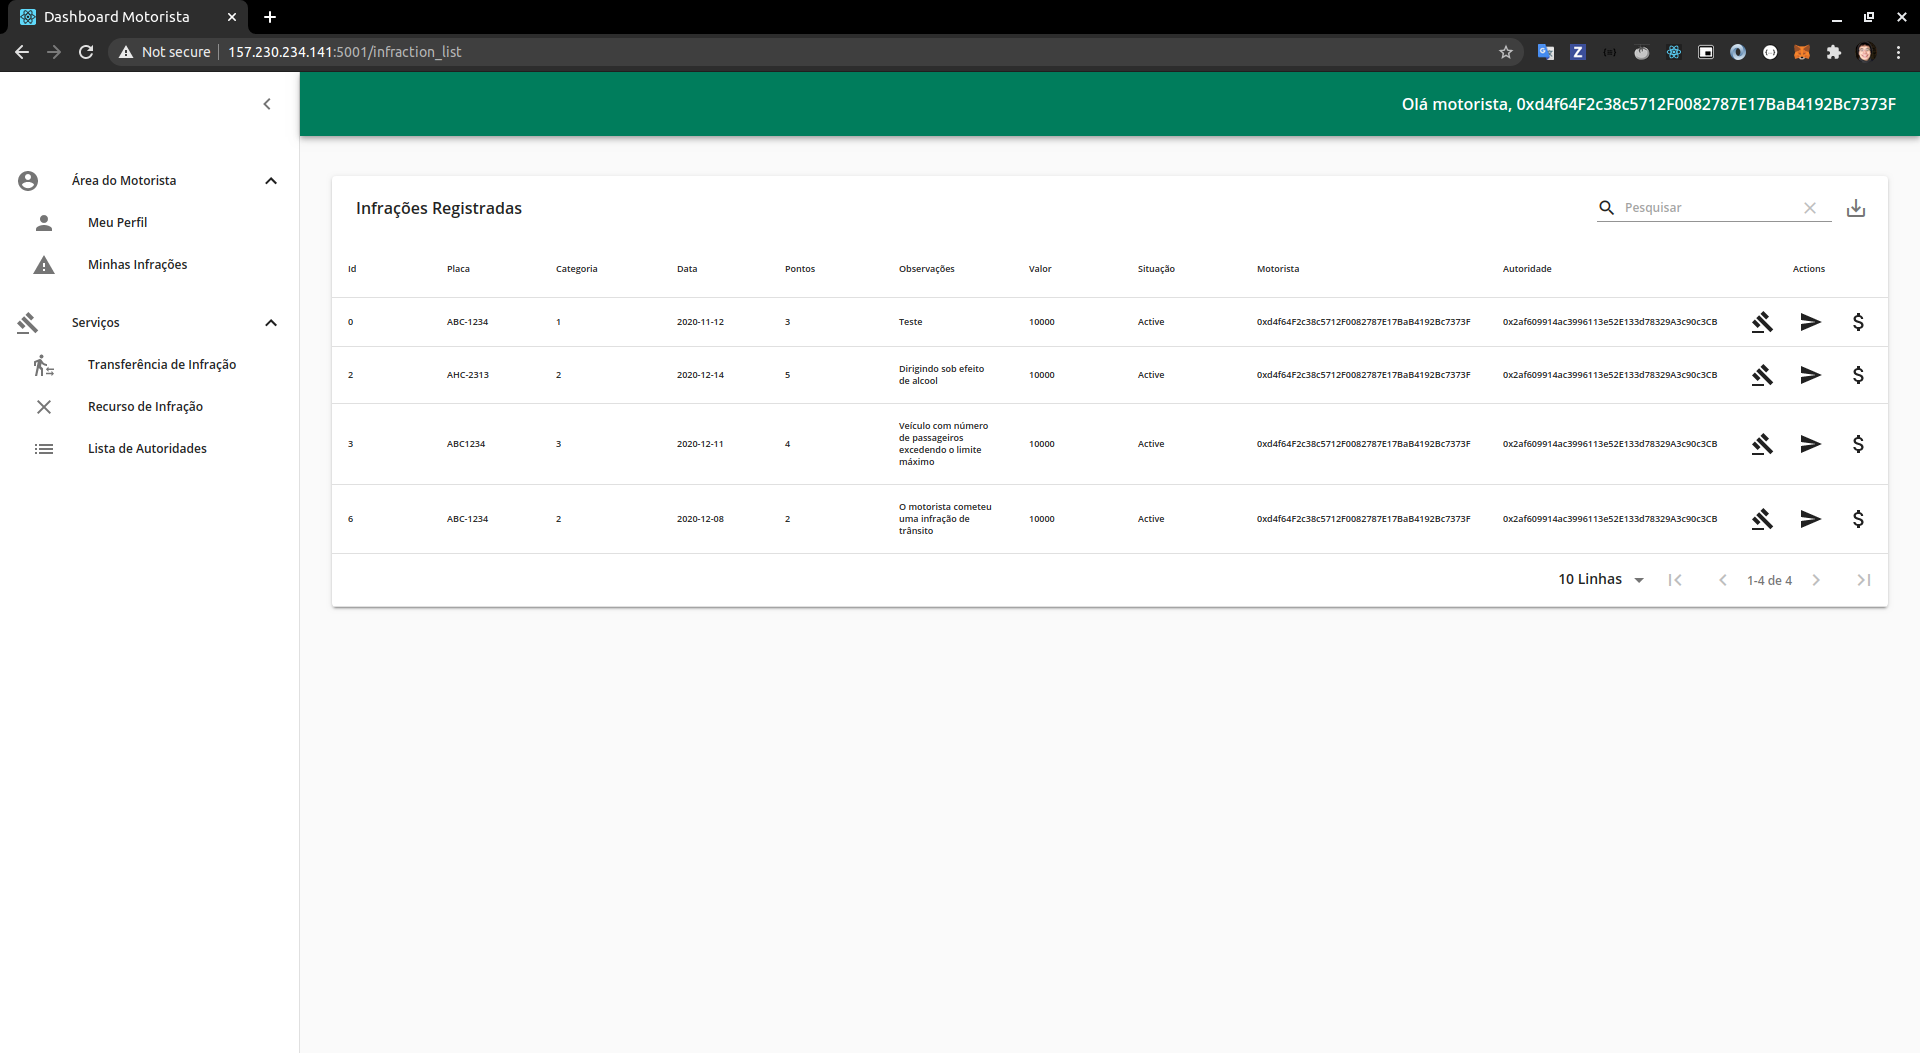
\includegraphics[scale=0.2]{figuras/capitulo_5/registro/print_7.png}
         \caption{Infração registrada e listada para o motorista infrator no módulo de motoristas}
         \label{fig:dapp_rede_ethereum}
    \end{figure}
    
Para visualizar o funcionamento das outras funcionalidades presentes no sistema assim como especificações de seu funcionamento acesse o vídeo disponível em \url{https://www.youtube.com/watch?v=Q1qknimuyW8}. Ou execute uma instância local da aplicação utilizando o código fonte disponibilizado na Seção \ref{sec:github}.
    
\section{Considerações acerca da solução}

O módulo cliente desenvolvido é um protótipo que busca validar o desenvolvimento de uma solução ao problema utilizando aplicações descentralizadas dentro da rede Ethereum. Naturalmente, alguns cuidados necessários a aplicações em produção não foram implementados neste momento, porém que não devem ser desconsiderados na utilização do mesmo em outros contextos.

A solução atual não contempla:

    \begin{quote}
        \begin{itemize}
            \item Requisitos de acessibilidade, não sendo totalmente acessível a navegação por meio de teclado ou leitores de tela;
            \item As aplicações descentralizadas no momento são executadas sob um protocolo HTTP dentro do servidor, sendo necessária em caso de utilização fora do contexto de validação a utilização do protocolo HTTPS;
             \item Atualmente o contrato está disponível para utilização em uma Rede Pública de testes e a configuração das aplicações foi feita para este caso. Se desejar utilizar a aplicação cliente em outra rede diferente da Ropsten Testnet é necessário que se altere essa configuração dentro do arquivo Infraction.json dentro do código fonte de cada aplicação;
        \end{itemize}
    \end{quote}
    

\subsection{Segurança das bibliotecas e ferramentas utilizadas}

Para o desenvolvimento da solução foram utilizadas algumas ferramentas e bibliotecas de terceiros, elencadas na Seção \ref{sec:tecnologias_ferramentas}, e algumas considerações a cerca da segurança das mesmas precisam ser feitas. A aplicação desenvolvida traz uma segurança e confiabilidade nos dados utilizando-se da tecnologia blockchain, porém também se torna necessário que os módulos da aplicação cliente também sigam critérios de segurança computacional para garantir que a solução como um todo seja segura para uso.

A segurança da aplicação cliente está diretamente ligada as ferramentas e bibliotecas utilizadas para sua construção, assim como os aspectos de implementação. A seguir serão feitas algumas considerações a cerca da segurança destes elementos e a sua utilização na aplicação.

\subsubsection{ReactJS}

O ReactJS é uma biblioteca para criação de interfaces de usuário, sendo uma das bibliotecas mais utilizadas ao redor do mundo para a criação de aplicações web. Seu desenvolvimento é feito de forma open-source, tendo uma grande comunidade ativa evoluindo sua implementação e corrigindo vulnerabilidades quando encontradas trazendo confiabilidade por parte de quem a utiliza, porém é necessário que o desenvolvedor tome alguns cuidados durante a implementação para garantir que as informações estão seguras de possíveis ameaças. O \citeauthor{uppLabs_securityReactjs} elenca alguns dos riscos mais comuns para aplicações web e aplicações que utilizam o ReactJS, e entre eles temos: \textit{Cross-site Scripting}, \textit{SQL Injection}, estado inicial controlado pelo atacante de renderização do lado do servidor, execução arbitrária de código, etc.

Além de alguns dos problemas mais comuns de segurança entre as aplicações o \citeauthor{uppLabs_securityReactjs} também traz algumas boas práticas para a segurança de aplicações ReactJS, e entre as boas práticas temos:

    \begin{quote}
        \begin{itemize}
            \item Como defesa contra vulnerabilidades de XSS, remova ou desative qualquer marcação que possa conter instruções para executar o código. Para HTML, isso inclui elementos como <script>, <object>, <embed> e <link>.
            \item Implemente Idle Timeout na aplicação React.
             \item Use bibliotecas de snippet como ES7 React, Redux, JS Snippets, etc. Eles trarão segurança adicional e manterão seu código livre de bugs.
             \item Explore falhas de injeção de script nos aplicativos.
             \item O código deve se comportar conforme o esperado e deve ser facilmente testável. É recomendado nomear seus arquivos de teste como os arquivos de origem com um sufixo .test.
             \item Limpe todo o aplicativo React durante e após o processo de desenvolvimento para capturar todos os ataques DDoS de vários tipos.
             \item Teste a funcionalidade de cada componente da aplicação e teste seu aplicativo completo assim que ele é renderizado no navegador.
        \end{itemize}
    \end{quote}
    
Como pode-se notar a segurança da aplicação cliente que utiliza ReactJS para sua construção é obtida a partir de aspectos de segurança computacional implementados dentro da biblioteca assim como boas práticas por parte do desenvolvedor durante a construção da mesma. A solução implementada neste trabalho leva em conta somente alguns destes aspectos em sua implementação pois se trata de um protótipo, o que torna necessário que ao se utilizar este trabalho em um contexto de produção os aspectos citados anteriormente sejam revisados e implementados caso não estejam presentes.

\subsubsection{Web3}

O Web3, como dito anteriormente, é uma coleção de bibliotecas que permitem que você interaja com um nó Ethereum local ou remoto usando HTTP, IPC ou WebSocket. A sua construção também é feita de forma open-source, assim como o ReactJS, tendo um grande comunidade verificando e agindo para corrigir vulnerabilidades encontradas.

Na versão mais atual desta biblioteca até o momento (1.3.1) existe uma vulnerabilidade conhecida que foi reportada pelo \citeauthor{snyk_web3vulnerabilities}, uma plataforma de desenvolvedores focada em construir aplicações com segurança, sendo descrita como: 

 \begin{quotation}
 "As versões afetadas deste pacote são vulneráveis ao armazenamento inseguro de credenciais. A implementação atual do web3.js pode resultar na descriptografia da carteira em certas circunstâncias. Quando uma carteira é salva e criptografada no armazenamento local, uma chave privada é necessária para carregar a carteira. No entanto, essa chave privada está disponível via \textit{LocalStorage} e pode ser lida em texto simples em uma página da web depois que uma carteira é carregada.
 
Essa implementação pode ser abusada por um invasor por meio de ataques do lado do cliente, como \textit{Cross-site Scripting} (XSS), e pode resultar no roubo da chave privada da carteira de um usuário."

 \end{quotation}

Para que essa vulnerabilidade presente nesta versão da biblioteca utilizada no projeto não seja explorada por um atacante é necessário que mecanismos de segurança sejam implementados na aplicação cliente que a utiliza. Evitando assim que os ataques no cliente possam explorá-la até que uma correção seja publicada em uma versão subsequente da biblioteca.

\subsubsection{Metamask}

O Metamask tem a confiança de mais de um milhões de usuários por todo mundo, sendo essa uma das mais carteiras Ethereum mais populares assim como é considerada uma das melhores disponíveis. Porém o que torna essa carteira segura além da confiabilidade por parte da comunidade que a utiliza?

\citeauthor{metamask_eran} cita que a carteira MetaMask é uma carteira sem custódia, interagindo diretamente com o blockchain Ethereum. Ele define que uma carteira sem custódia é um tipo de carteira descentralizada, em que o cliente possui suas chaves privadas, onde ao configurar o MetaMask, o usuário obtém um arquivo com as chaves privadas e precisa escrever uma frase-semente com a qual poderá restaurar seus fundos, onde ter chaves privadas significa que você tem controle total sobre os fundos. 

Ele também cita que em seu artigo que para maior segurança, MetaMask suporta carteiras de hardware (como Ledger e Trezor): carteiras de hardware podem proteger seus fundos mesmo no caso de uma invasão do computador, tornando a MetaMask uma das opções mais seguras disponíveis. 

Porém \citeauthor{metamask_aaron} cita em seu artigo que um risco ao se utilizar carteiras como a Metamask é o ataque de phishing, um tipo de ataque onde o atacante busca roubar informações pessoais como senhas. Ele descreve que este ataque poderia ocorrer da seguinte forma: 

 \begin{quotation}
"Gene está trabalhando em seu laptop com várias guias abertas em seu navegador. Ele desbloqueia sua carteira MetaMask para fazer uma transação. Um invasor usa as guias abertas para ver se Gene está usando MetaMask.

O invasor envia a Gene uma mensagem pop-up dizendo que sua transação falhou. Isso acontece às vezes, então Gene não está preocupado. Ele insere sua senha para refazer a transação. O invasor agora tem acesso à carteira de Gene."

 \end{quotation}
 
 Logo em seguida \citeauthor{metamask_aaron} também traz mais informações sobre o assunto relatando que este tipo de ataque é bastante comum em carteiras online e que a equipe do Metamask está trabalhando em patches para este tipo de problema. Dizendo também que ao utilizar carteiras virtuais os usuários são responsáveis por sua própria segurança, trazendo a recomendação de que se use apenas uma guia por vez para fazer transações e mantenha a carteira bloqueada quando não a estiver usando.

\subsubsection{Docker e Docker-compose}

Os contêineres são utilizados para facilitar o gerenciamento de dependências da aplicação assim como orquestrar facilmente os ambientes de desenvolvimento e produção das mesmas. Neste projeto essas ferramentas são utilizadas para facilitar a utilização dos dois ambientes, facilitando a geração de build dos módulos da aplicação cliente e consequentemente o deploy das mesmas no servidor em que estão hospedadas.

\citeauthor{docker_vulnerabilities} traz em seu artigo algumas vulnerabilidades comuns a contêineres que devem ser observadas e mitigadas pelos desenvolvedores. A seguir vamos elencar algumas:

    \begin{quote}
        \begin{itemize}
            \item Criptojacking: Criptojacking é um tipo de ataque em que um script malicioso é usado para roubar os recursos computacionais de um dispositivo para minerar criptomoedas. Os contêineres podem ser suscetíveis a criptojacking se contiverem imagens maliciosas que dão aos invasores acesso root a todo o contêiner. Eles também são vulneráveis se os endpoints da API do docker container estiverem publicamente acessíveis na Internet sem senhas ou firewalls de segurança.
            \item Imagens maliciosas de código aberto: É uma vulnerabilidade que torna possível sobrescrever o binário runc do host dá aos atacantes a margem de manobra para executar comandos com acesso root. Os mecanismos Docker anteriores à v18.09.2 tornam os contêineres com imagens controladas pelo invasor suscetíveis à vulnerabilidade CVE-2019-5736. Os utilizadores são aconselhados, tanto quanto possível, a fazer uso de imagens oficiais do Docker fornecidas.
            \item Dockerfiles estáticos: Um dos princípios dos contêineres é que uma imagem é imutável. Isso significa que, quando uma imagem é construída, seu conteúdo é imutável. Isso por si só dá origem a vulnerabilidades que resultam de pacotes/bibliotecas/imagens desatualizados contidos em uma imagem. Portanto, é uma boa ideia incorporar scanners de vulnerabilidade em processos de CI / CD para identificar imagens de contêiner vulneráveis. Como as imagens são imutáveis, lançar um contêiner recém-criado com dependências atualizadas ajudará a conter as vulnerabilidades de segurança, pois a correção do contêiner é desencorajada.
        \end{itemize}
    \end{quote}

Neste projeto foram utilizadas as bibliotecas em suas versões mais recentes de forma a mitigar problemas de segurança, imagens oficiais disponibilizadas pela equipe Docker, assim como somente as portas necessárias de cada aplicação são liberadas para acesso externo na configuração dos contêineres. Recomenda-se em uma utilização posterior da aplicação que essas dependências sejam verificadas e atualizadas caso necessário, criando-se assim uma nova imagem com essas atualizações.

\subsubsection{Solidity}

Em toda a linguagem de programação aspectos de segurança devem ser levados em conta e adotados durante a utilização. No Solidity, isso é ainda mais importante porque você pode usar contratos inteligentes para lidar com tokens ou, possivelmente, coisas ainda mais valiosas onde as ações podem ser irreversíveis. Além disso, toda execução de um contrato inteligente acontece em público e, além disso, o código-fonte costuma estar disponível.

A documentação oficial da linguagem traz uma lista de recomendações para os desenvolvedores assim como uma explanação a cerca de mecanismos existentes na linguagem que podem ser utilizados nos contratos de forma a garantir a segurança em sua utilização. Estas recomendações podem ser acessadas em \url{https://docs.soliditylang.org/en/v0.6.12/security-considerations.html}.




\section{Acesso a implementação da solução}
\label{sec:github}

A solução foi desenvolvida em cima de ferramentas gratuitas e open source, assim como o código fonte utilizado para criação dos Dapps e o código do contrato estão regidos sob a licença GPL3 sendo assim gratuita a sua utilização.

Os arquivos fonte desta solução podem ser encontrados no repositório:  \url{https://github.com/joaopaulonsoares/aplicacaotccblockchain}.

Para dúvidas a cerca da implementação, entre em contato no email paulonsoares18@gmail.com ou criando uma Issue no repositório do Github citado anteriormente.

